\chapter{Evaluation} % (fold)
\label{cha:Evaluation}

We enjoyed making the game. Creating the game was frustrating, because it took really long to get a working version. When we finally had a working game, we enjoyed playing it, despite the horrible frame rate.

\section{Problems with the current set-up} % (fold)
\label{sec:problems_with_the_current_set_up}

This was the first time OGO 3.1 was given in 1 semester. We have found a few problems with the way the project was organized:

\begin{itemize}
    \item Too much time was planned for the design document. We wasted a lot of time making small changes to the design, changes which, during implementation, often turned out not to matter, not to be as good as the original, or not to be implemented at all due to time constraints. 
    \item There was too little time for actually making the game. A lot of errors in the game were found after the presentation. If we had 2 more weeks, we would have finished the game. 
\end{itemize}

te veel tijd voor design document
te weinig tijd voor code

% section problems_with_the_current_set_up (end)

\section{Peer reviews} % (fold)
\label{sec:peer_reviews}

At the last meeting with our tutor, Stef van den Elzen, we made anonymous peer reviews Below is 

\begin{table}[h!t!]

    \begin{tabular}{l|l}
        \hline
        Person                      & Comments \\
        \hline
        Leroy Bakker                & Goed inzet getoont mbt openGL \\
        Etienne van Delden          & Goed aanwezig en houdt het overzicht\\
        Edin Dudojevic              & Minder discussieren, meer accepteren en coden \\
                                    & Af en toe lang discussieren over dingen die al besloten zijn\\
                                    & Minder praten, meer coden\\
                                    & Erg veel commentaar vaak\\
                                    & Ging af en toe te diep op dingen in\\
        Neal van den Eerthwegh      & Duidelijker aangeven wat je doet/wilt\\
        Jeroen Habraken             & Minder op IRC zitten\\
        Stef Louwers                & Goed ingezet\\
        Anson van Rooij             & Goed de groep er bij gehouden \\
        \hline
    \end{tabular}
        \caption{Outcomes of Peer reviews}
        \label{table:definitions}
\end{table}

\begin{figure}[!ht]
  \centering
  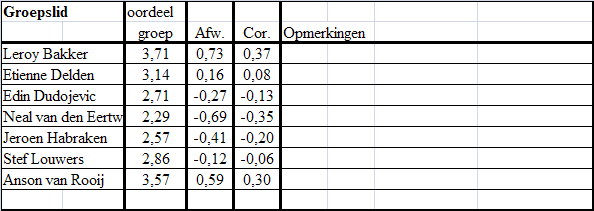
\includegraphics[width=12cm,height=5cm]{diagrams/groep2}
  \caption{The group evaluation} \label{fig:modules}
\end{figure}

% section peer_reviews (end)



% chapter Evaluation (end) 